%%%%%%%%%%%%%%%%%%%%%%%%%%%%%%%%%%%%%%%%%%%%%%%%%%%%%%%%%%%%%%%%%%%%%%%%%%%%%%%%
%2345678901234567890123456789012345678901234567890123456789012345678901234567890
%        1         2         3         4         5         6         7         8

\documentclass[letterpaper, 12 pt, conference]{ieeeconf}  % Comment this line out
                                                          % if you need a4paper
%\documentclass[a4paper, 10pt, conference]{ieeeconf}      % Use this line for a4
\usepackage{graphicx}
\graphicspath{ {images/} }% paper
\usepackage{amsmath}
\usepackage{algorithm}
\usepackage{array}
\usepackage{tabu}
\usepackage{siunitx}
\usepackage{booktabs}% for better rules in the table
%\usepackage[ruled]{algorithm2e}

\usepackage[noend]{algpseudocode}
\makeatletter
\def\BState{\State\hskip-\ALG@thistlm}
\makeatother
\IEEEoverridecommandlockouts                              % This command is only
\usepackage{mathtools}
\DeclarePairedDelimiter{\ceil}{\lceil}{\rceil}                                                          % needed if you want to
                                                          % use the \thanks command
\overrideIEEEmargins
% See the \addtolength command later in the file to balance the column lengths
% on the last page of the document

\title{\LARGE 
IDAA432C Assignment-5 (Group: 41)
}

\author{
  Aditya Vallabh\\
  \texttt{IIT2016517}
  \and
  Kiran Velumuri\\
  \texttt{ITM2016009}
  \and
  Neil Syiemlieh\\
  \texttt{IIT2016125}
  \and
  Tauhid Alam\\
  \texttt{BIM2015003}
}


\begin{document}



\maketitle
\thispagestyle{empty}
\pagestyle{empty}


%%%%%%%%%%%%%%%%%%%%%%%%%%%%%%%%%%%%%%%%%%%%%%%%%%%%%%%%%%%%%%%%%%%%%%%%%%%%%%%%

\subsection*{ \textbf{Question} }
\textbf{Write an efficient algorithm which, given an inorder traversal, can construct a corresponding complete binary tree. Do the necessary experimentation and analysis with your algorithm. }


%%%%%%%%%%%%%%%%%%%%%%%%%%%%%%%%%%%%%%%%%%%%%%%%%%%%%%%%%%%%%%%%%%%%%%%%%%%%%%%%
\section{Introduction}
The problem requires us to construct a complete binary tree given the inorder traversal. In theory, there can be many possible trees with the same inorder traversal but the problem statement mentions we need to to construct a complete binary tree. Such a tree, however, would be unique and we have implemented an algorithm to do the same.

\section{Algorithm Design}
\subsection{Complete Binary Tree}
A complete binary tree is a binary tree in which every level,  except possibly the last, is completely filled, and all nodes in the last level are as far left as possible. Sometimes it is also referrred to as an almost complete binary tree.


\subsection{Array Traversal}
A Complete Binary Tree can be easily represented as array and array based representation is space efficient. If the parent node is stored at index $I$ (0-indexed)
\begin{enumerate}
\item The left child will be at $2 * I + 1$
\item The right child will be at $2 * I + 2$
\end{enumerate}

\begin{figure}[H]
\includegraphics[scale=0.6]{arrayRepr}
\caption{Array representation for a heap (1-based indexing)}
\end{figure}

\subsection{Main Method}
\begin{algorithm}[H]
\caption{Main Method}\label{alg:main}
\begin{algorithmic}
\Procedure{main}{}
\State Input: $arr, n$
\State $buildTree(arr, tree, 0, n)$
\State $print(tree)$
\State $inorder(tree, 0, n)$
\EndProcedure
\end{algorithmic}
\end{algorithm}
In the main method, we first take the inorder traversal array size and the array as the input. Then we call the $buildTree()$ function to convert the inorder traversal to a complete binary tree and store it in another array called $tree$. Then we verify the inorder traversal by calling the $inorder()$ function which performs the inorder traversal on the complete binary tree.

\subsection{Build Tree}
An almost complete binary tree can be represented as an array. So this algorithm basically converts the given inorder traversal to an almost completely filled binary tree.
\begin{algorithm}[H]
\caption{buildTree Algorithm}\label{alg:buildTree}
\begin{algorithmic}
\State $k \gets 0$
\Procedure{buildTree}{arr, tree, i, n}
\If {$i < n$}
  \State $buildTree(arr, tree, 2*i + 1, n)$
  \State $tree[i] \gets arr[k]$
  \State $k \gets k + 1$
  \State $buildTree(arr, tree, 2*i + 2, n)$
\EndIf
\EndProcedure
\end{algorithmic}
\end{algorithm}
In this algorithm we recursively insert the elements in the tree in the following fashion:
\begin{enumerate}
\item Build the left sub-tree
\item Insert the root element
\item Build the right sub-tree
\end{enumerate}
Here the insertion occurs in the same order as the given inorder traversal array. This way, we'll construct an almost complete binary tree which has the same inorder traversal as the given array.

\subsection{Inorder Traversal}
\begin{algorithm}[H]
\caption{Inorder Traversal Algorithm}\label{alg:inorder}
\begin{algorithmic}
\Procedure{inorder}{arr, i, n}
\If {$i < n$}
  \State $inorder(arr, 2*i + 1, n)$
  \State $print(arr[i])$
  \State $inorder(arr, 2*i + 2, n)$
\EndIf
\EndProcedure
\end{algorithmic}
\end{algorithm}
In this kind of traversal we recursively print the elements of the tree in the following fashion:
\begin{enumerate}
\item Traverse left sub-tree
\item Print the root element
\item Traverse the right sub-tree
\end{enumerate}
This prints the inorder traversal of any given complete binary tree.

\section{Analysis and Discussion}
\subsection{Time Complexity}
A binary tree in-order traversal can be described by the following recurrence relation, where $T(n)$ is the time taken to traverse on a complete binary tree of size $n$.
\begin{align*}
&T(n) = 2\ T(\frac{n}{2}) + O(1) \\
&T(1) = O(1)
\end{align*}
Here, the $T(\frac{n}{2})$ is for the traversal of both subtrees from the current node and the $O(1)$ is for the current node. We can solve the recurrence relation as follows:
\begin{align*}
T(n) &= 2\ T(\frac{n}{2}) + 1 \\
&= 2\ [2\ T(\frac{n}{4}) + 1] + 1 \\
&= 4\ T(\frac{n}{4}) + 3 \\
&= 4\ [2\ T(\frac{n}{8}) + 1] + 3 \\
&\vdots \\
T(n) &= 2^k\ T(\frac{n}{2^k}) + (2^k - 1)
\end{align*}
For\ $T(1)$:
\begin{align*}
&\implies \frac{n}{2^k} = 1 \\
&\implies 2^k = n
\end{align*}
Entering the value of $2^k$ in the equation above, we obtain the solution:
\begin{align*}
T(n) = 2n - 1
\end{align*}
Hence, the time complexity of the algorithm is $O(n)$. There is no notion of best, average or worst case, because the computation time depends solely on the size of the input, not the values of the input elements.

\subsection{Space Complexity}
We are using the array representation of an almost complete binary tree hence for a tree containing n elements, we would require only n nodes. Hence the space complexity of our algorithm is $O(n)$.

\section{Experimental Analysis}
The algorithm was run against various inputs randomly generated for $n$ ranging from 1 to 1000. The total number of computations have been plotted against the size of the input in Fig. 1.
\begin{figure}[H]
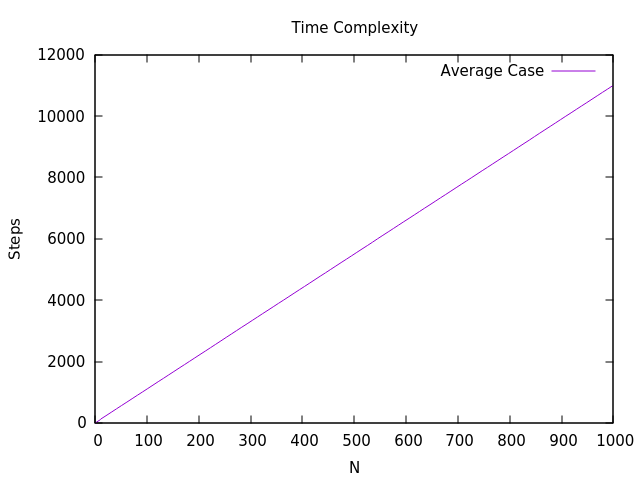
\includegraphics[scale=0.65]{inorder}
\caption{Time complexity of constructing the binary tree}
\end{figure}
We see that the graph is linear, which is expected as the time complexity of the algorithm is O(n) where n is the size of inorder traversal.

\subsection{Discussion}
We have implemented an algorithm which converts the inorder traversal into an almost complete binary tree with a complexity of $O(n)$. This is the best complexity one can achieve because given $n$ elements, each one has to be inserted in the tree. Each insertion takes $O(1)$ time. So $n$ insertions would take:
\begin{align*}
n*O(1) = O(n)
\end{align*}
Therefore the minimum complexity one can achieve is $O(n)$ and we have done that in this paper.

\section{Conclusion}
Through this paper we proposed the algorithm to construct an almost complete binary tree from the given inorder traversal. Moreover our algorithm has both time and space complexities of $O(n)$.
The inorder traversal is a compact form to store a completely filled binary tree. A tree is generally stored as a group of nodes where each node contains a key and the pointers to its children. This implementation takes at lest thrice the space taken by an array. So we have used the array representation.


\begin{thebibliography}{99}

\bibitem{c1} Introduction to Algorithms
Book by Charles E. Leiserson, Clifford Stein, Ronald Rivest, and Thomas H. Cormen
\end{thebibliography}

\end{document}
